%\VignetteIndexEntry{Introduction to the dataRetrieval package}
%\VignetteDepends{}
%\VignetteSuggests{}
%\VignetteImports{}
%\VignettePackage{}

\documentclass[a4paper,11pt]{article}

\usepackage{amsmath}
\usepackage{times}
\usepackage{hyperref}
\usepackage[numbers, round]{natbib}
\usepackage[american]{babel}
\usepackage{authblk}
\renewcommand\Affilfont{\itshape\small}
\usepackage{Sweave}
\renewcommand{\topfraction}{0.85}
\renewcommand{\textfraction}{0.1}
\usepackage{graphicx}


\textwidth=6.2in
\textheight=8.5in
\parskip=.3cm
\oddsidemargin=.1in
\evensidemargin=.1in
\headheight=-.3in

%------------------------------------------------------------
% newcommand
%------------------------------------------------------------
\newcommand{\scscst}{\scriptscriptstyle}
\newcommand{\scst}{\scriptstyle}
\newcommand{\Robject}[1]{{\texttt{#1}}}
\newcommand{\Rfunction}[1]{{\texttt{#1}}}
\newcommand{\Rclass}[1]{\textit{#1}}
\newcommand{\Rpackage}[1]{\textit{#1}}
\newcommand{\Rexpression}[1]{\texttt{#1}}
\newcommand{\Rmethod}[1]{{\texttt{#1}}}
\newcommand{\Rfunarg}[1]{{\texttt{#1}}}

\begin{document}
\Sconcordance{concordance:dataRetrieval.tex:dataRetrieval.Rnw:%
1 126 1 49 0 1 7 15 1 1 14 55 1 3 0 36 1 2 0 11 1 24 %
0 24 1 3 0 23 1 3 0 6 1 7 0 18 1 3 0 25 1 1 0 17 1 9 %
0 6 1 7 0 21 1 8 0 16 1 2 0 11 1 23 0 21 1 9 0 20 1 3 %
0 6 1 17 0 27 1 6 0 11 1 9 0 15 1 20 0 21 1 4 0 21 1 %
4 0 17 1 7 0 22 1 8 0 19 1 4 0 9 1 4 0 78 1 1 2 9 1 1 %
4 4 1 20 0 44 1 4 0 32 1 4 0 21 1 4 0 21 1 37 0 13 1 %
9 0 95 1 4 0 9 1 12 0 13 1 4 0 14 1 4 0 5 1 4 0 23 1 %
18 0 8 1 4 0 55 1}


%------------------------------------------------------------
\title{Introduction to the dataRetrieval package}
%------------------------------------------------------------
\author[1]{Laura De Cicco}
\author[1]{Robert Hirsch}
\affil[1]{United States Geological Survey}



\maketitle
\tableofcontents

%------------------------------------------------------------
\section{Introduction to dataRetrieval}
%------------------------------------------------------------ 
The dataRetrieval package was created to simplify the process of getting hydrologic data in the R enviornment. It has been specifically designed to work seamlessly with the EGRET package: Exploration and Graphics for RivEr Trends (EGRET). See: \url{https://github.com/USGS-R/EGRET/wiki} for information on EGRET.

There is a plethora of hydrological data available on the web. This package is designed specifically to load United States Geological Survey (USGS) hydrologic data to the R enviornment. This includes daily values, real-time (unit values), site information, and water quality sample data. 

%------------------------------------------------------------ 
\section{Getting Started}
%------------------------------------------------------------ 
This section describes the options for downloading and installing the dataRetrieval package.
%------------------------------------------------------------
\subsection{New to R?}
%------------------------------------------------------------ 
If you are new to R, you will need to first install the latest version of R, which can be found here: \url{http://www.r-project.org/}.

There are many options for running and editing R code, one nice enviornment to learn R is RStudio. RStudio can be downloaded here: \url{http://rstudio.org/}. Once R and RStudio are installed, the dataRetrieval package needs to be installed as described in the next section.

%------------------------------------------------------------
\subsection{R User: Installing dataRetrieval from downloaded binary}
%------------------------------------------------------------ 
The latest dataRetrieval package build is available for download at \url{https://github.com/USGS-R/dataRetrieval/blob/master/dataRetrieval_1.2.1.tar.gz}.  If the package's tar.gz file is saved in R's working directory, then the following command will fully install the package:

\begin{Schunk}
\begin{Sinput}
> install.packages("dataRetrieval_1.2.1.tar.gz", 
+                  repos=NULL, type="source")
\end{Sinput}
\end{Schunk}

If the downloaded file is stored in an alternative location, include the path in the install command.  A Windows example looks like this (notice the direction of the slashes, they are in the opposite direction that Windows normally creates paths):

\begin{Schunk}
\begin{Sinput}
> install.packages(
+   "C:/RPackages/Statistics/dataRetrieval_1.2.1.tar.gz", 
+   repos=NULL, type="source")
\end{Sinput}
\end{Schunk}

A Mac example looks like this:

\begin{Schunk}
\begin{Sinput}
> install.packages(
+   "/Users/userA/RPackages/Statistic/dataRetrieval_1.2.1.tar.gz", 
+   repos=NULL, type="source")
\end{Sinput}
\end{Schunk}

It is a good idea to re-start the R enviornment after installing the package, especially if installing an updated version (that is, restart RStudio). Some users have found it necessary to delete the previous version's package folder before installing newer version of dataRetrieval. If you are experiencing issues after updating a package, trying deleting the package folder - the default location for Windows is something like this: C:/Users/userA/Documents/R/win-library/2.15/dataRetrieval, and the default for a Mac: /Users/userA/Library/R/2.15/library/dataRetrieval. Then, re-install the package using the directions above. Moving to CRAN should solve this problem.

After installing the package, you need to open the library each time you re-start R.  This is done with the simple command:
\begin{Schunk}
\begin{Sinput}
> library(dataRetrieval)
\end{Sinput}
\end{Schunk}
Using RStudio, you could alternatively click on the checkbox for dataRetrieval in the Packages window.

%------------------------------------------------------------
\subsection{R Developers: Installing dataRetrieval from gitHub}
%------------------------------------------------------------
Alternatively, R-developers can install the latest version of dataRetrieval directly from gitHub using the devtools package.  devtools is available on CRAN.  Simpley type the following commands into R to install the latest version of dataRetrieval available on gitHub.  Rtools (for Windows) and latex tools are required.

\begin{Schunk}
\begin{Sinput}
> library(devtools)
> install_github("dataRetrieval", "USGS-R")
\end{Sinput}
\end{Schunk}
To then open the library, simply type:

\begin{Schunk}
\begin{Sinput}
> library(dataRetrieval)
\end{Sinput}
\end{Schunk}

\newpage
%------------------------------------------------------------
\section{Raw Data: USGS Web Retrieval Examples}
%------------------------------------------------------------ 
In this section, we will run through 5 examples, documenting how to get raw data from the web. This includes historical daily values, real-time current values, water quality data, site information, and measured parameter information. 
%------------------------------------------------------------
\subsection{USGS Web Retrieval Introduction}
%------------------------------------------------------------
The United States Geological Survey organizes their hydrological data in fairly standard structure.  Gage stations are located throughout the United States, each station has a unique ID.  Often (but not always), these ID's are 8 digits.  The first step to finding data is discoving this 8-digit ID. One potential tool for discovering data is Environmental Data Discovery and Transformation (EnDDaT): \url{http://cida.usgs.gov/enddat/}.  Follow the example in the User's Guide to learn how to discover USGS stations and available data from any location in the United States. Essentially, you can create a Project Location on the map, set a bounding box (in miles), then search for USGS Time Series and USGS Water Quality Data. Locations, ID's, available data, and available time periods will load on the map and appropriate tabs.

Once the site-ID is known, the next required input for USGS data retrievals is the 'parameter code'.  This is a 5-digit code that specifies what measured paramater is being requested.  A complete list of possible USGS parameter codes can be found here: 

\url{http://nwis.waterdata.usgs.gov/usa/nwis/pmcodes?radio_pm_search=param_group&pm_group=All+--+include+all+parameter+groups&pm_search=&casrn_search=&srsname_search=&format=html_table&show=parameter_group_nm&show=parameter_nm&show=casrn&show=srsname&show=parameter_units}

Not every station will measure all parameters. The following is a list of commonly measured parameters:

% latex table generated in R 2.15.2 by xtable 1.7-0 package
% Wed Jan 23 14:59:25 2013
\begin{table}[ht]
\begin{center}
\caption{Commonly found USGS Parameter Codes}
\begin{tabular}{rll}
  \hline
 & pCode & shortName \\ 
  \hline
1 & 00060 & Discharge [cfs] \\ 
  2 & 00065 & Gage height [ft] \\ 
  3 & 00010 & Temperature [C] \\ 
  4 & 00045 & Precipitation [in] \\ 
  5 & 00400 & pH \\ 
   \hline
\end{tabular}
\end{center}
\end{table}
For real-time data, the parameter code and site ID will suffice.  The USGS stores historical data as daily values however.  The statistical process used to store the daily data is the final requirement for daily value retrievals.  A 5-digit 'stat code' specifies the requested processing.  A complete list of possible USGS stat codes can be found here:

\url{http://nwis.waterdata.usgs.gov/nwis/help/?read_file=stat&format=table}

The most common stat codes are:
% latex table generated in R 2.15.2 by xtable 1.7-0 package
% Wed Jan 23 14:59:25 2013
\begin{table}[ht]
\begin{center}
\caption{Commonly found USGS Stat Codes}
\begin{tabular}{rll}
  \hline
 & StatCode & shortName \\ 
  \hline
1 & 00001 & Maximum \\ 
  2 & 00002 & Minimum \\ 
  3 & 00003 & Mean \\ 
  4 & 00008 & Median \\ 
   \hline
\end{tabular}
\end{center}
\end{table}

We will use the Choptank River near Greensboro, MD as an example.  The site-ID for this gage station is 01491000. Daily discharge measurements are available as far back as 1948.  Additionally, forms of nitrate and nitrogen have been measured dating back to 1964.

%------------------------------------------------------------
\subsection{USGS Daily Value Retrievals}
%------------------------------------------------------------
To obtain historic daily records of USGS data, use the retrieveNWISData function. The arguments for this function are siteNumber, parameterCd, startDate, endDate, statCd, and a logical (true/false) interactive. There are 2 default argument: statCd defaults to "00003" and interactive defaults to TRUE.  If you want to use the default values, you do not need to list them in the function call. Setting the 'interactive' option to true will walk you through the function. It might make more sense to run large batch collections with the interactive option set to FALSE. 

The dates (start and end) need to be in the format "YYYY-MM-DD".  Setting the start date to "" will indicate to the program to ask for the earliest date, setting the end date to "" will ask for the latest available date.

\begin{Schunk}
\begin{Sinput}
> # Using defaults:
> siteNumber <- "01491000" # Site ID for Choptank River near Greensboro, MD
> parameterCd <- "00060"  # Discharge in cubic feet per second
> startDate <- ""
> endDate <- ""
> discharge <- retrieveNWISData(siteNumber, parameterCd, startDate, endDate)
\end{Sinput}
\end{Schunk}

A dataframe is returned that looks like the following:
\begin{Schunk}
\begin{Soutput}
  agency_cd  site_no   datetime X02_00060_00003 X02_00060_00003_cd
1      USGS 01491000 1948-01-01             190                  A
2      USGS 01491000 1948-01-02             900                  A
3      USGS 01491000 1948-01-03             480                  A
4      USGS 01491000 1948-01-04             210                  A
5      USGS 01491000 1948-01-05             210                  A
6      USGS 01491000 1948-01-06             220                  A
\end{Soutput}
\end{Schunk}
The structure of the dataframe is:
\begin{Schunk}
\begin{Soutput}
'data.frame':	23764 obs. of  5 variables:
 $ agency_cd         : chr  "USGS" "USGS" "USGS" "USGS" ...
 $ site_no           : chr  "01491000" "01491000" "01491000" "01491000" ...
 $ datetime          : Date, format: "1948-01-01" "1948-01-02" ...
 $ X02_00060_00003   : num  190 900 480 210 210 220 160 130 120 100 ...
 $ X02_00060_00003_cd: chr  "A" "A" "A" "A" ...
\end{Soutput}
\end{Schunk}
Note that dateTime is automatically imported as a Date. Each requested parameter has a value and remark code column.  The names of these columns depend on the requested parameter and stat code combinations. USGS remark codes are often "A" (approved for publication) or "P" (provisional data subject to revision). A more complete list of remark codes can be found here:
\url{http://waterdata.usgs.gov/usa/nwis/help?codes_help}

Another example that doesn't use the defaults would be a request for mean and maximum daily temperature and discharge in early 2012:
\begin{Schunk}
\begin{Sinput}
> # Using defaults:
> siteNumber <- "01491000" # Site ID for Choptank River near Greensboro, MD
> parameterCd <- "00010,00060"  # Temperature and discharge
> statCd <- "00001,00003"  #mean and maximum
> startDate <- "2012-01-01"
> endDate <- "2012-06-30"
> temperatureAndFlow <- retrieveNWISData(siteNumber, parameterCd, 
+                   startDate, endDate, StatCd=statCd,interactive=FALSE)
\end{Sinput}
\end{Schunk}

Daily data is pulled from \url{http://waterservices.usgs.gov/rest/DV-Test-Tool.html}. 

An example of plotting the above data:
\begin{Schunk}
\begin{Sinput}
> par(mar=c(5,4,4,5)+.1)
> with(temperatureAndFlow, plot(
+   datetime, X01_00010_00003,
+   xlab="Date",ylab="Temperature [C]"
+   ))
> par(new=TRUE)
> with(temperatureAndFlow, plot(
+   datetime, X02_00060_00003,
+   col="red",type="l",xaxt="n",yaxt="n",xlab="",ylab="",axes=FALSE
+   ))
> axis(4,col="red",col.axis="red")
> mtext("Discharge [cfs]",side=4,line=3,col="red")
\end{Sinput}
\end{Schunk}
\begin{figure}
\begin{center}
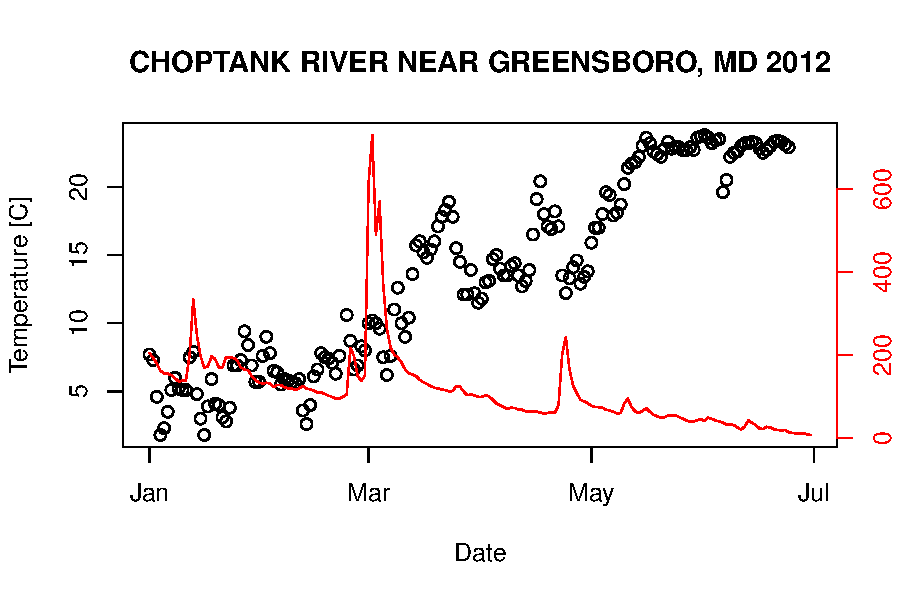
\includegraphics{dataRetrieval-fig1}
\end{center}
\caption{Temperature and discharge plot of Choptank River.}
\end{figure}

There are occasions where NWIS values are not reported as numbers, instead there might be text describing a certain event such as "Ice".  Any value that cannot be converted to a number will be reported as NA in this package.

%------------------------------------------------------------
\subsection{USGS Unit Value Retrievals}
%------------------------------------------------------------
We can also get real-time, instantaneous measurements using the retrieveUnitNWISData function:
\begin{Schunk}
\begin{Sinput}
> # Using defaults:
> siteNumber <- "01491000" # Site ID for Choptank River near Greensboro, MD
> parameterCd <- "00060"  # Discharge in cubic feet per second
> startDate <- as.character(Sys.Date())
> endDate <- as.character(Sys.Date())
> dischargeToday <- retrieveUnitNWISData(siteNumber, parameterCd, startDate, endDate)
\end{Sinput}
\end{Schunk}
Which produces the following dataframe:
\begin{Schunk}
\begin{Soutput}
  agency_cd  site_no            datetime tz_cd X02_00060 X02_00060_cd
1      USGS 01491000 2013-01-23 00:00:00   EST       190            P
2      USGS 01491000 2013-01-23 00:15:00   EST       187            P
3      USGS 01491000 2013-01-23 00:30:00   EST       187            P
4      USGS 01491000 2013-01-23 00:45:00   EST       187            P
5      USGS 01491000 2013-01-23 01:00:00   EST       192            P
6      USGS 01491000 2013-01-23 01:15:00   EST       187            P
\end{Soutput}
\end{Schunk}
The structure of the dataframe is:
\begin{Schunk}
\begin{Soutput}
'data.frame':	62 obs. of  6 variables:
 $ agency_cd   : chr  "USGS" "USGS" "USGS" "USGS" ...
 $ site_no     : chr  "01491000" "01491000" "01491000" "01491000" ...
 $ datetime    : POSIXct, format: "2013-01-23 00:00:00" "2013-01-23 00:15:00" ...
 $ tz_cd       : chr  "EST" "EST" "EST" "EST" ...
 $ X02_00060   : num  190 187 187 187 192 187 192 187 187 187 ...
 $ X02_00060_cd: chr  "P" "P" "P" "P" ...
\end{Soutput}
\end{Schunk}
Note that time now becomes important, so the dateTime is a POSIXct, and the time zone is included. Data is pulled from \url{http://waterservices.usgs.gov/rest/IV-Test-Tool.html}. There are occasions where NWIS values are not reported as numbers, instead a common example is "Ice".  Any value that cannot be converted to a number will be reported as NA in this package.

%------------------------------------------------------------
\subsection{USGS Water Quality Retrievals}
%------------------------------------------------------------
Finally, we can use the dataRetrieval package to get water quality data that is available on the water quality data portal: \url{http://www.waterqualitydata.us/}. The function is getQWData, with the similar input arguments: siteNumber, parameterCd, startDate, endDate, and interactive. The difference is in parameterCd, in this function multiple parameters can be queried using a ";" separator, and setting parameterCd <- "" will return all of the measured observations.

\begin{Schunk}
\begin{Sinput}
> # Using defaults:
> siteNumber <- "01491000" # Site ID for Choptank River near Greensboro, MD
> parameterCd <- "00618;71851"  # Dissolved Nitrate parameter codes (one as mg/l as N, one as mg/l)
> startDate <- "1964-06-11"
> endDate <- "2012-12-18"
> dissolvedNitrate <- getRawQWData(siteNumber, parameterCd, startDate, endDate)
\end{Sinput}
\end{Schunk}

Producing a dataframe with the following columns:
\begin{Schunk}
\begin{Soutput}
 [1] "OrganizationIdentifier"                           
 [2] "OrganizationFormalName"                           
 [3] "ActivityIdentifier"                               
 [4] "ActivityTypeCode"                                 
 [5] "ActivityMediaName"                                
 [6] "ActivityMediaSubdivisionName"                     
 [7] "ActivityStartDate"                                
 [8] "ActivityStartTime.Time"                           
 [9] "ActivityStartTime.TimeZoneCode"                   
[10] "ActivityEndDate"                                  
[11] "ActivityEndTime.Time"                             
[12] "ActivityEndTime.TimeZoneCode"                     
[13] "ActivityDepthHeightMeasure.MeasureValue"          
[14] "ActivityDepthHeightMeasure.MeasureUnitCode"       
[15] "ActivityDepthAltitudeReferencePointText"          
[16] "ActivityTopDepthHeightMeasure.MeasureValue"       
[17] "ActivityTopDepthHeightMeasure.MeasureUnitCode"    
[18] "ActivityBottomDepthHeightMeasure.MeasureValue"    
[19] "ActivityBottomDepthHeightMeasure.MeasureUnitCode" 
[20] "ProjectIdentifier"                                
[21] "ActivityConductingOrganizationText"               
[22] "MonitoringLocationIdentifier"                     
[23] "ActivityCommentText"                              
[24] "SampleAquifer"                                    
[25] "HydrologicCondition"                              
[26] "HydrologicEvent"                                  
[27] "SampleCollectionMethod.MethodIdentifier"          
[28] "SampleCollectionMethod.MethodIdentifierContext"   
[29] "SampleCollectionMethod.MethodName"                
[30] "SampleCollectionEquipmentName"                    
[31] "ResultDetectionConditionText"                     
[32] "CharacteristicName"                               
[33] "ResultSampleFractionText"                         
[34] "ResultMeasureValue"                               
[35] "ResultMeasure.MeasureUnitCode"                    
[36] "MeasureQualifierCode"                             
[37] "ResultStatusIdentifier"                           
[38] "StatisticalBaseCode"                              
[39] "ResultValueTypeName"                              
[40] "ResultWeightBasisText"                            
[41] "ResultTimeBasisText"                              
[42] "ResultTemperatureBasisText"                       
[43] "ResultParticleSizeBasisText"                      
[44] "PrecisionValue"                                   
[45] "ResultCommentText"                                
[46] "USGSPCode"                                        
[47] "ResultDepthHeightMeasure.MeasureValue"            
[48] "ResultDepthHeightMeasure.MeasureUnitCode"         
[49] "ResultDepthAltitudeReferencePointText"            
[50] "SubjectTaxonomicName"                             
[51] "SampleTissueAnatomyName"                          
[52] "ResultAnalyticalMethod.MethodIdentifier"          
[53] "ResultAnalyticalMethod.MethodIdentifierContext"   
[54] "ResultAnalyticalMethod.MethodName"                
[55] "MethodDescriptionText"                            
[56] "LaboratoryName"                                   
[57] "AnalysisStartDate"                                
[58] "ResultLaboratoryCommentText"                      
[59] "DetectionQuantitationLimitTypeName"               
[60] "DetectionQuantitationLimitMeasure.MeasureValue"   
[61] "DetectionQuantitationLimitMeasure.MeasureUnitCode"
[62] "PreparationStartDate"                             
\end{Soutput}
\end{Schunk}

To get a simplified dataframe that contains only datetime, value, and qualifier, use the function getQWData:

\begin{Schunk}
\begin{Sinput}
> dissolvedNitrateSimple <- getQWData(siteNumber, parameterCd, startDate, endDate)
> head(dissolvedNitrateSimple)
\end{Sinput}
\begin{Soutput}
     dateTime qualifier.71851 value.71851 qualifier.00618 value.00618
1  1964-06-11                         3.3                       0.745
3  1964-09-10                         5.3                       1.200
5  1965-02-01                         2.9                       0.655
7  1965-02-25                         2.4                       0.542
9  1965-03-25                         1.5                       0.339
11 1965-04-20                         2.2                       0.497
\end{Soutput}
\end{Schunk}
Note that in this dataframe, datatime is only imported as Dates (no times are included), and the qualifier is either blank or "<" signifying a censored value.


%------------------------------------------------------------
\subsection{USGS Site Information Retrievals}
%------------------------------------------------------------
To obtain all of the available site information, use the getSiteFileData function:
\begin{Schunk}
\begin{Sinput}
> # Using defaults:
> siteNumber <- "01491000" # Site ID for Choptank River near Greensboro, MD
> ChopTankInfo <- getSiteFileData(siteNumber)
\end{Sinput}
\end{Schunk}

The available data for these for the USGS sites are:
\begin{Schunk}
\begin{Sinput}
> colnames(ChopTankInfo)
\end{Sinput}
\begin{Soutput}
 [1] "agency.cd"             "site.no"               "station.nm"           
 [4] "site.tp.cd"            "lat.va"                "long.va"              
 [7] "dec.lat.va"            "dec.long.va"           "coord.meth.cd"        
[10] "coord.acy.cd"          "coord.datum.cd"        "dec.coord.datum.cd"   
[13] "district.cd"           "state.cd"              "county.cd"            
[16] "country.cd"            "land.net.ds"           "map.nm"               
[19] "map.scale.fc"          "alt.va"                "alt.meth.cd"          
[22] "alt.acy.va"            "alt.datum.cd"          "huc.cd"               
[25] "basin.cd"              "topo.cd"               "instruments.cd"       
[28] "construction.dt"       "inventory.dt"          "drain.area.va"        
[31] "contrib.drain.area.va" "tz.cd"                 "local.time.fg"        
[34] "reliability.cd"        "gw.file.cd"            "nat.aqfr.cd"          
[37] "aqfr.cd"               "aqfr.type.cd"          "well.depth.va"        
[40] "hole.depth.va"         "depth.src.cd"          "project.no"           
[43] "queryTime"            
\end{Soutput}
\end{Schunk}
Pulling out a specific example piece of information, in this case station name can be done as follows:
\begin{Schunk}
\begin{Sinput}
> ChopTankInfo$station.nm
\end{Sinput}
\begin{Soutput}
[1] "CHOPTANK RIVER NEAR GREENSBORO, MD"
\end{Soutput}
\end{Schunk}
Site information is obtained from \url{http://waterservices.usgs.gov/rest/Site-Test-Tool.html}

%------------------------------------------------------------
\subsection{USGS Parameter Information Retrievals}
%------------------------------------------------------------
To obtain all of the available information concerning a measured parameter, use the getParameterInfo function:
\begin{Schunk}
\begin{Sinput}
> # Using defaults:
> parameterCd <- "00618" 
> parameterINFO <- getParameterInfo(parameterCd)
\end{Sinput}
\end{Schunk}

The available data for these for the USGS sites are:
\begin{Schunk}
\begin{Sinput}
> colnames(parameterINFO)
\end{Sinput}
\begin{Soutput}
[1] "parameter_cd"       "parameter_group_nm" "parameter_nm"      
[4] "casrn"              "srsname"            "parameter_units"   
\end{Soutput}
\end{Schunk}
Pulling out a specific example piece of information, in this case station name can be done as follows:
\begin{Schunk}
\begin{Sinput}
> parameterINFO$parameter_nm
\end{Sinput}
\begin{Soutput}
[1] "Nitrate, water, filtered, milligrams per liter as nitrogen"
\end{Soutput}
\end{Schunk}
Parameter information is obtained from \url{http://nwis.waterdata.usgs.gov/nwis/pmcodes/}


%------------------------------------------------------------
\section{Polished Data: USGS Web Retrieval Examples}
%------------------------------------------------------------ 
In this example, we use 3 dataRetrieval functions to get daily streamflow data and inorganic nitrogen sample results, and site information for a USGS gaging station with the ID 06934500.  The station is Missouri River at Hermann, MO (which is discovered in the INFO dataset). Rather than see the raw output from NWIS, we will get more polished returned data frames.  These data frames were exclusively designed to work with the EGRET R package, however can be very useful for all hydrologic studies.


\begin{Schunk}
\begin{Sinput}
> Daily <- getDVData("06934500","00060","1970-10-01","2011-09-30")
\end{Sinput}
\begin{Soutput}
There are  14975 data points, and  14975 days.
There are  0 zero flow days
If there are any zero discharge days, all days had 0 cubic meters per second added to the discharge value.
\end{Soutput}
\begin{Sinput}
> head(Daily)
\end{Sinput}
\begin{Soutput}
        Date        Q Julian Month Day  DecYear MonthSeq Qualifier i     LogQ
1 1970-10-01 3879.408  44102    10 274 1970.747     1450         A 1 8.263438
2 1970-10-02 3454.655  44103    10 275 1970.750     1450         A 2 8.147478
3 1970-10-03 3029.903  44104    10 276 1970.753     1450         A 3 8.016286
4 1970-10-04 2644.793  44105    10 277 1970.755     1450         A 4 7.880348
5 1970-10-05 2293.665  44106    10 278 1970.758     1450         A 5 7.737906
6 1970-10-06 2072.793  44107    10 279 1970.761     1450         A 6 7.636652
  Q7 Q30
1 NA  NA
2 NA  NA
3 NA  NA
4 NA  NA
5 NA  NA
6 NA  NA
\end{Soutput}
\begin{Sinput}
> Sample <-getSampleData("06934500","00631","1970-10-01","2011-09-30")
> head(Sample)
\end{Sinput}
\begin{Soutput}
        Date ConcLow ConcHigh Uncen ConcAve Julian Month Day  DecYear MonthSeq
1 1979-09-26    1.10     1.10     1    1.10  47384     9 269 1979.734     1557
2 1979-10-16    0.42     0.42     1    0.42  47404    10 289 1979.788     1558
3 1979-11-27    2.00     2.00     1    2.00  47446    11 331 1979.903     1559
4 1979-12-18    1.70     1.70     1    1.70  47467    12 352 1979.960     1560
5 1980-01-29    1.30     1.30     1    1.30  47509     1  29 1980.078     1561
6 1980-02-21    1.10     1.10     1    1.10  47532     2  52 1980.141     1562
       SinDY      CosDY
1 -0.9946999 -0.1028210
2 -0.9712570  0.2380333
3 -0.5724040  0.8199718
4 -0.2463613  0.9691781
5  0.4699767  0.8826788
6  0.7733507  0.6339785
\end{Soutput}
\begin{Sinput}
> INFO <-getMetaData("06934500","00631", interactive=FALSE)
> colnames(INFO)
\end{Sinput}
\begin{Soutput}
 [1] "agency.cd"             "site.no"               "station.nm"           
 [4] "site.tp.cd"            "lat.va"                "long.va"              
 [7] "dec.lat.va"            "dec.long.va"           "coord.meth.cd"        
[10] "coord.acy.cd"          "coord.datum.cd"        "dec.coord.datum.cd"   
[13] "district.cd"           "state.cd"              "county.cd"            
[16] "country.cd"            "map.nm"                "map.scale.fc"         
[19] "alt.va"                "alt.meth.cd"           "alt.acy.va"           
[22] "alt.datum.cd"          "huc.cd"                "basin.cd"             
[25] "topo.cd"               "construction.dt"       "inventory.dt"         
[28] "drain.area.va"         "contrib.drain.area.va" "tz.cd"                
[31] "local.time.fg"         "reliability.cd"        "project.no"           
[34] "queryTime"             "drainSqKm"             "staAbbrev"            
[37] "param.nm"              "param.units"           "paramShortName"       
[40] "paramNumber"           "constitAbbrev"        
\end{Soutput}
\begin{Sinput}
> INFO$station.nm
\end{Sinput}
\begin{Soutput}
[1] "Missouri River at Hermann, MO"
\end{Soutput}
\begin{Sinput}
> Sample <- mergeReport()
\end{Sinput}
\begin{Soutput}
 Discharge Record is 14975 days long, which is 41 years
 First day of the discharge record is 1970-10-01 and last day is 2011-09-30
 The water quality record has 437 samples
 The first sample is from 1979-09-26 and the last sample is from 2011-09-29
 Discharge: Minimum, mean and maximum 394 2660 20900
 Concentration: Minimum, mean and maximum 0.02 1.3 4.2
 Percentage of the sample values that are censored is 1.4 %
\end{Soutput}
\end{Schunk}

\newpage

%------------------------------------------------------------
% BIBLIO
%------------------------------------------------------------
\begin{thebibliography}{10}

\bibitem{HirschI}
Helsel, D.R. and R. M. Hirsch, 2002. Statistical Methods in Water Resources Techniques of Water Resources Investigations, Book 4, chapter A3. U.S. Geological Survey. 522 pages. \url{http://pubs.usgs.gov/twri/twri4a3/}

\bibitem{HirschII}
Hirsch, R. M., Moyer, D. L. and Archfield, S. A. (2010), Weighted Regressions on Time, Discharge, and Season (WRTDS), with an Application to Chesapeake Bay River Inputs. JAWRA Journal of the American Water Resources Association, 46: 857-880. doi: 10.1111/j.1752-1688.2010.00482.x \url{http://onlinelibrary.wiley.com/doi/10.1111/j.1752-1688.2010.00482.x/full}

\bibitem{HirschIII}
Sprague, L. A., Hirsch, R. M., and Aulenbach, B. T. (2011), Nitrate in the Mississippi River and Its Tributaries, 1980 to 2008: Are We Making Progress? Environmental Science \& Technology, 45 (17): 7209-7216. doi: 10.1021/es201221s \url{http://pubs.acs.org/doi/abs/10.1021/es201221s}

\end{thebibliography}

\end{document}

\end{document}
